% Options for packages loaded elsewhere
\PassOptionsToPackage{unicode}{hyperref}
\PassOptionsToPackage{hyphens}{url}
%
\documentclass[
]{article}
\usepackage{lmodern}
\usepackage{amssymb,amsmath}
\usepackage{ifxetex,ifluatex}
\ifnum 0\ifxetex 1\fi\ifluatex 1\fi=0 % if pdftex
  \usepackage[T1]{fontenc}
  \usepackage[utf8]{inputenc}
  \usepackage{textcomp} % provide euro and other symbols
\else % if luatex or xetex
  \usepackage{unicode-math}
  \defaultfontfeatures{Scale=MatchLowercase}
  \defaultfontfeatures[\rmfamily]{Ligatures=TeX,Scale=1}
\fi
% Use upquote if available, for straight quotes in verbatim environments
\IfFileExists{upquote.sty}{\usepackage{upquote}}{}
\IfFileExists{microtype.sty}{% use microtype if available
  \usepackage[]{microtype}
  \UseMicrotypeSet[protrusion]{basicmath} % disable protrusion for tt fonts
}{}
\makeatletter
\@ifundefined{KOMAClassName}{% if non-KOMA class
  \IfFileExists{parskip.sty}{%
    \usepackage{parskip}
  }{% else
    \setlength{\parindent}{0pt}
    \setlength{\parskip}{6pt plus 2pt minus 1pt}}
}{% if KOMA class
  \KOMAoptions{parskip=half}}
\makeatother
\usepackage{xcolor}
\IfFileExists{xurl.sty}{\usepackage{xurl}}{} % add URL line breaks if available
\IfFileExists{bookmark.sty}{\usepackage{bookmark}}{\usepackage{hyperref}}
\hypersetup{
  pdftitle={Quantified Self Report},
  pdfauthor={Abhisek Gautam},
  hidelinks,
  pdfcreator={LaTeX via pandoc}}
\urlstyle{same} % disable monospaced font for URLs
\usepackage[margin=1in]{geometry}
\usepackage{color}
\usepackage{fancyvrb}
\newcommand{\VerbBar}{|}
\newcommand{\VERB}{\Verb[commandchars=\\\{\}]}
\DefineVerbatimEnvironment{Highlighting}{Verbatim}{commandchars=\\\{\}}
% Add ',fontsize=\small' for more characters per line
\usepackage{framed}
\definecolor{shadecolor}{RGB}{248,248,248}
\newenvironment{Shaded}{\begin{snugshade}}{\end{snugshade}}
\newcommand{\AlertTok}[1]{\textcolor[rgb]{0.94,0.16,0.16}{#1}}
\newcommand{\AnnotationTok}[1]{\textcolor[rgb]{0.56,0.35,0.01}{\textbf{\textit{#1}}}}
\newcommand{\AttributeTok}[1]{\textcolor[rgb]{0.77,0.63,0.00}{#1}}
\newcommand{\BaseNTok}[1]{\textcolor[rgb]{0.00,0.00,0.81}{#1}}
\newcommand{\BuiltInTok}[1]{#1}
\newcommand{\CharTok}[1]{\textcolor[rgb]{0.31,0.60,0.02}{#1}}
\newcommand{\CommentTok}[1]{\textcolor[rgb]{0.56,0.35,0.01}{\textit{#1}}}
\newcommand{\CommentVarTok}[1]{\textcolor[rgb]{0.56,0.35,0.01}{\textbf{\textit{#1}}}}
\newcommand{\ConstantTok}[1]{\textcolor[rgb]{0.00,0.00,0.00}{#1}}
\newcommand{\ControlFlowTok}[1]{\textcolor[rgb]{0.13,0.29,0.53}{\textbf{#1}}}
\newcommand{\DataTypeTok}[1]{\textcolor[rgb]{0.13,0.29,0.53}{#1}}
\newcommand{\DecValTok}[1]{\textcolor[rgb]{0.00,0.00,0.81}{#1}}
\newcommand{\DocumentationTok}[1]{\textcolor[rgb]{0.56,0.35,0.01}{\textbf{\textit{#1}}}}
\newcommand{\ErrorTok}[1]{\textcolor[rgb]{0.64,0.00,0.00}{\textbf{#1}}}
\newcommand{\ExtensionTok}[1]{#1}
\newcommand{\FloatTok}[1]{\textcolor[rgb]{0.00,0.00,0.81}{#1}}
\newcommand{\FunctionTok}[1]{\textcolor[rgb]{0.00,0.00,0.00}{#1}}
\newcommand{\ImportTok}[1]{#1}
\newcommand{\InformationTok}[1]{\textcolor[rgb]{0.56,0.35,0.01}{\textbf{\textit{#1}}}}
\newcommand{\KeywordTok}[1]{\textcolor[rgb]{0.13,0.29,0.53}{\textbf{#1}}}
\newcommand{\NormalTok}[1]{#1}
\newcommand{\OperatorTok}[1]{\textcolor[rgb]{0.81,0.36,0.00}{\textbf{#1}}}
\newcommand{\OtherTok}[1]{\textcolor[rgb]{0.56,0.35,0.01}{#1}}
\newcommand{\PreprocessorTok}[1]{\textcolor[rgb]{0.56,0.35,0.01}{\textit{#1}}}
\newcommand{\RegionMarkerTok}[1]{#1}
\newcommand{\SpecialCharTok}[1]{\textcolor[rgb]{0.00,0.00,0.00}{#1}}
\newcommand{\SpecialStringTok}[1]{\textcolor[rgb]{0.31,0.60,0.02}{#1}}
\newcommand{\StringTok}[1]{\textcolor[rgb]{0.31,0.60,0.02}{#1}}
\newcommand{\VariableTok}[1]{\textcolor[rgb]{0.00,0.00,0.00}{#1}}
\newcommand{\VerbatimStringTok}[1]{\textcolor[rgb]{0.31,0.60,0.02}{#1}}
\newcommand{\WarningTok}[1]{\textcolor[rgb]{0.56,0.35,0.01}{\textbf{\textit{#1}}}}
\usepackage{graphicx,grffile}
\makeatletter
\def\maxwidth{\ifdim\Gin@nat@width>\linewidth\linewidth\else\Gin@nat@width\fi}
\def\maxheight{\ifdim\Gin@nat@height>\textheight\textheight\else\Gin@nat@height\fi}
\makeatother
% Scale images if necessary, so that they will not overflow the page
% margins by default, and it is still possible to overwrite the defaults
% using explicit options in \includegraphics[width, height, ...]{}
\setkeys{Gin}{width=\maxwidth,height=\maxheight,keepaspectratio}
% Set default figure placement to htbp
\makeatletter
\def\fps@figure{htbp}
\makeatother
\setlength{\emergencystretch}{3em} % prevent overfull lines
\providecommand{\tightlist}{%
  \setlength{\itemsep}{0pt}\setlength{\parskip}{0pt}}
\setcounter{secnumdepth}{-\maxdimen} % remove section numbering

\title{Quantified Self Report}
\author{Abhisek Gautam}
\date{23/09/2019}

\begin{document}
\maketitle

\begin{Shaded}
\begin{Highlighting}[]
\NormalTok{knitr}\OperatorTok{::}\NormalTok{opts_knit}\OperatorTok{$}\KeywordTok{set}\NormalTok{(}\DataTypeTok{root.dir =} \StringTok{'images'}\NormalTok{)}
\end{Highlighting}
\end{Shaded}

\hypertarget{introduction}{%
\section{1. Introduction}\label{introduction}}

Quantified Self (QS), a word coined in the year 2008 by a group of
researchers and data enthusiasts has had a large number of followers
since its introduction(Ferris, 2013). The primary motive of the
philosophy is to gather data and analyse them to justify one's
behaviour, trends and habits so that one can change his/her behaviour so
that he/she can lead a better life. The term QS is defined as
``Quantified Self (QS) is the term that embodies self-knowledge through
self-tracking'' (Quantified Self Institute, 2017).

Our team, InnoData started collecting three types of data which could be
used to check some behaviours that we had as a group. The types of data
that were collected are as follows:

\begin{itemize}
\tightlist
\item
  GPS Data
\item
  Mood Data
\item
  Steps Count
\item
  Messages (Individual Data)
\item
  Rainfall (External Data)
\end{itemize}

In addition to that, two more datasets had been added, viz.~my social
media usage for my individual analysis and publicly available rainfall
data of Sydney.

With these data, we wanted to answer three questions in our group:

\begin{enumerate}
\def\labelenumi{\arabic{enumi}.}
\tightlist
\item
  Who in the group has travelled the most in Sydney?
\item
  Does happiness relate with steps count?
\item
  Who in the group prefers to walk and who doesn't?
\end{enumerate}

Some of the questions for my individual analysis are as follows:

\begin{enumerate}
\def\labelenumi{\arabic{enumi}.}
\tightlist
\item
  Whether I used more social media on weekends, when I don't have work?
\item
  Does my social media usage relate with my number of steps?
\end{enumerate}

This report is made on the basis of the data that was collected in the
period of six weeks.

\hypertarget{collection-of-data}{%
\section{2. Collection of Data}\label{collection-of-data}}

Our group started with brainstorming the types of data that could be
collected easily and accurately. We decided to collect our GPS data,
emotions, steps and call log history. We agreed using WhatsApp as our
mode of communication and use Google drive to share our data. Our data
was collected from 4th of August 2019 till 14th of September 2019. The
process of collection of our group data is described below.

\hypertarget{gps}{%
\subsection{2.1 GPS}\label{gps}}

GPS data was readily available in all our smartphones, and its bulk
could be downloaded from Google. Luckily, all of the team members had
Android Smartphone, hence this data would be available for all. We
agreed to have GPS location tracking enabled at all times. This data
gave an account of our GPS positions at different times of the day.

\hypertarget{mood}{%
\subsection{2.2 Mood}\label{mood}}

For getting the mood data, we would take selfies at random times of the
day and process them in a facial recognition software. Initially, we
used an app called Feely, available on Play Store to get the emotions of
individual photos. However, the results that were given by the app was
not clear, so we switched to using Microsoft Azure API to calculate
emotions. We would have eight emotions associated with the selfie photos
now, as well as the datetime the photo was taken.

\hypertarget{steps-count}{%
\subsection{2.3 Steps Count}\label{steps-count}}

Initially, we decided to use an app called Pedometer to count our steps.
Later on we found out that Google itself tracks our steps via Google Fit
app. So, all of us switched from Pedometer to using Google's Google Fit
app. The data also could be downloaded from Google.

\hypertarget{individual-data--messages-in-messenger}{%
\subsection{2.4 Individual Data- Messages in
Messenger}\label{individual-data--messages-in-messenger}}

Facebook's Messenger data was collected to check my social media usage
as it is the app that I use the most. The data could be extracted from
Facebook for the period of this study.

\hypertarget{external-data--weather}{%
\subsection{2.5 External Data- Weather}\label{external-data--weather}}

Weather has a lot of affects in the movement of people. Hence, weather
data of a station in Sydney was taken. Only daily rain was taken into
account. The data is taken from Australian Government's Bureau of
Meteorology website, from the Sydney Observatory Hill weather station
(``\url{http://www.bom.gov.au/climate/data/index.shtml?bookmark=136}'').

\hypertarget{data-processing-and-quality-issues}{%
\section{3. Data Processing and Quality
Issues}\label{data-processing-and-quality-issues}}

All of the members of our group had shared their data in the Google
drive. We then analysed individual data and tried to find out the issues
that were prevalent in the collected data.

\hypertarget{gps-1}{%
\subsection{3.1 GPS}\label{gps-1}}

As our GPS was tracked by our smartphones, it was consistent and in
detail. It records our GPS in regular intervals of time in a day, in KML
format. The data was extracted and loaded in the dataframe, and was
visualized by plotting in the map of Sydney. There were some outliers in
the data, which may have been caused by inaccurate reading. From the
Figure 1, we can see that there are some positions where GPS tracking
had fluctuated and recorded random data some times. Additionally, the
GPS data needed to be converted to standard datetime format so that it
could be compared with data tracked on the basis of date and time.

\begin{center}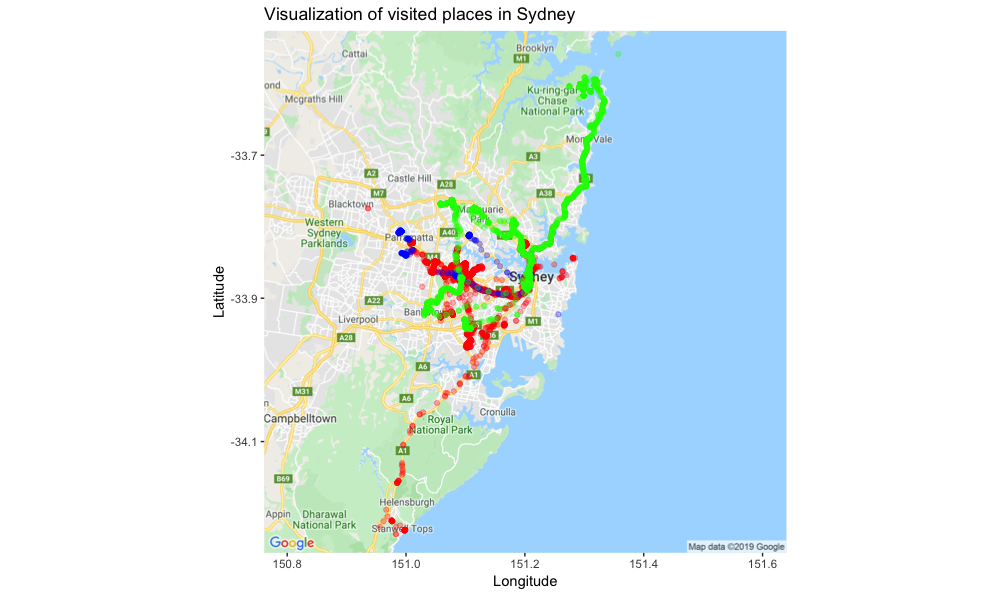
\includegraphics[width=1\linewidth]{/Users/abhisekgautam/Desktop/UTS/DSI/AT2//Location History All} \end{center}

\begin{figure}

{\centering 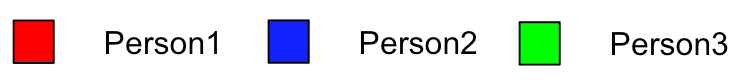
\includegraphics[width=0.3\linewidth]{/Users/abhisekgautam/Desktop/UTS/DSI/AT2//label} 

}

\caption{\label{fig:figs}Figure 1: Location History of All Group Members}\label{fig:add_picture93}
\end{figure}

\hypertarget{mood-1}{%
\subsection{3.2 Mood}\label{mood-1}}

In the mood data, there were issues of consistency and error in reading
the data. Here, we dealt with data inconsistency; as in some days, there
were no photos taken, and some days had multiple photos. We had
anticipated that the selfies would have a varying mood, but in reality,
everyone was giving their neutral reaction while clicking their selfies
So, besides a few photos, all of the moods returned by the mood
detection API were seen to be on the neutral spectrum and hence we
figured that this was inefficient to determine the mood of a person
processing selfies.

\hypertarget{steps-count-1}{%
\subsection{3.3 Steps Count}\label{steps-count-1}}

For steps count, that the application that was used to track steps
counted step even when we were not moving and sometimes it did not track
any. Also, we don't always carry our smartphones while walking, making
this data somewhat inaccurate. Using FitBit devices would have helped
overcoming the issues regarding inaccurate step count and it would have
given more accurate readings.

\hypertarget{messenger}{%
\subsection{3.4 Messenger}\label{messenger}}

For individual data, Facebook's messenger data gave the messages that
were sent and received by me. Messenger, being my primary chatting
application, would give a fair estimate of my social media usage.
However, deleted conversations could not be obtained. The time of this
data was converted to AEDT (Australian Eastern Daylight Time), and the
number of messages sent per day was counted.

\begin{figure}

{\centering 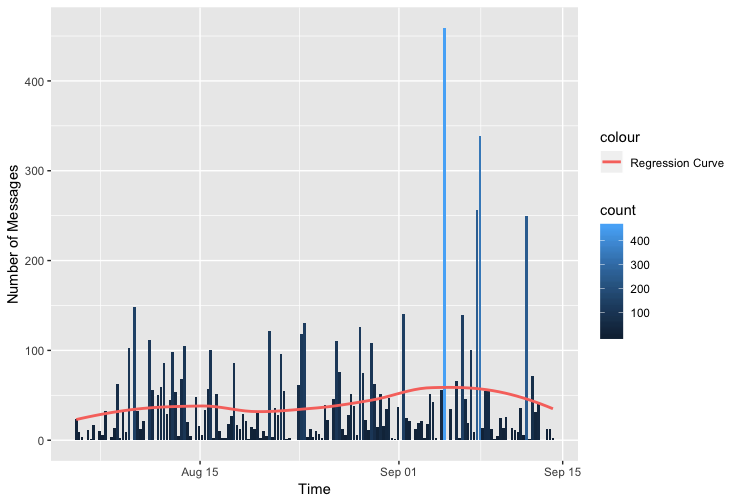
\includegraphics[width=0.8\linewidth]{/Users/abhisekgautam/Desktop/UTS/DSI/AT2//Messages_plot} 

}

\caption{\label{fig:figs}Figure 2: Plot showing Messages sent and received}\label{fig:add_picture2}
\end{figure}

\hypertarget{rainfall}{%
\subsection{3.5 Rainfall}\label{rainfall}}

The consideration with weather data was that if it showed rainfall, it
was assumed for the entire region of Sydney. This is not accurate as one
region may experience rainfall while another area may have a sunny
weather. However, since the Sydney Observatory Hill weather station is
located in the heart of Sydney, it was considered a fair assumption.

\begin{figure}

{\centering 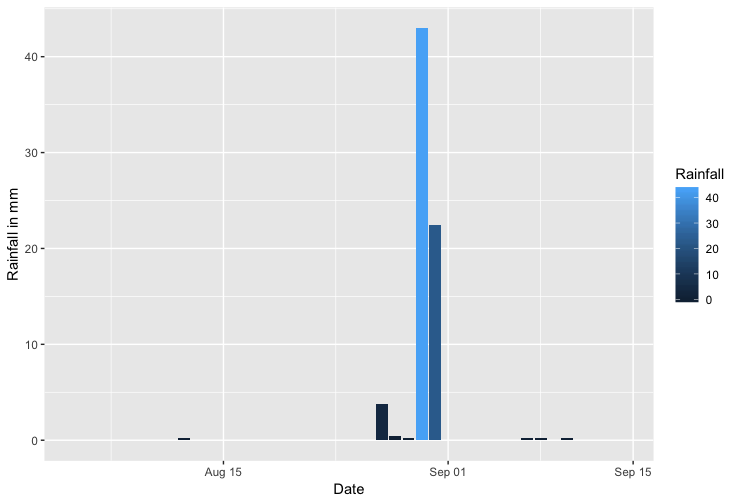
\includegraphics[width=0.6\linewidth]{/Users/abhisekgautam/Desktop/UTS/DSI/AT2//Rainfall} 

}

\caption{\label{fig:figs}Figure 3: Visualization of Rainfall Data}\label{fig:add_picture3}
\end{figure}

\hypertarget{analysis-and-insights}{%
\section{4. Analysis and Insights}\label{analysis-and-insights}}

The obtained data is charted using R's plotting functions keeping in
mind our initial questions. Analysis of the plots are done and insights
are formulated accordingly.

\hypertarget{gps-2}{%
\subsection{4.1 GPS}\label{gps-2}}

Looking at GPS data for the entire period of 6 weeks, from Figure 1,
Person3 had explored Sydney the most.

Furthermore, GPS data was analysed for a day that when all of us had
class; on 26th August 2019. On that day, the graph showed that all of
the members had been in the University Area, so all of them had attended
the class. With further inspection, it can be assumed that, Members 1
and 3 had come to the University and returned from the Central Station.
Member 2 also has also got a GPS point registered close to the station
but is not clear. Recollecting the happenings of that day, I remember
that all of us had come to the University differently and had returned
together via Central station.

\begin{center}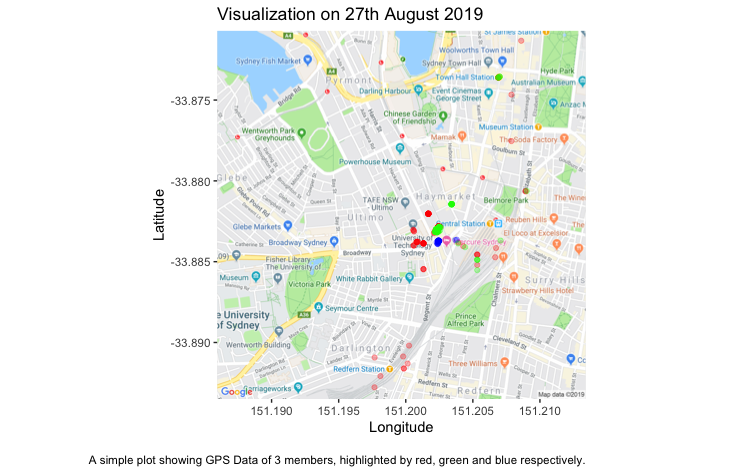
\includegraphics[width=0.8\linewidth]{/Users/abhisekgautam/Desktop/UTS/DSI/AT2//Uni Visit 27 Aug DSI Class} \end{center}

\begin{figure}

{\centering 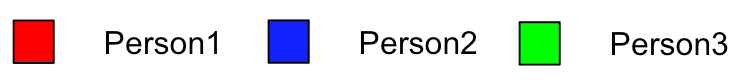
\includegraphics[width=0.3\linewidth]{/Users/abhisekgautam/Desktop/UTS/DSI/AT2//label} 

}

\caption{\label{fig:figs}Figure 4: Visualization showing GPS data of 27th August, 2019}\label{fig:add_picture91}
\end{figure}

\hypertarget{steps}{%
\subsection{4.2 Steps}\label{steps}}

Figure 5 shows that Person3 walks the most in the group.

Further, we see that the number of steps by all the members is most in
the Week 4 from Figure 5, which is from 26th August to 1st September.
Recollecting that week, it was because that week all three of us had
classes of three subjects; Statistical Thinking, Data Science and
Innovation and Data Science Practice. All of us were present on all
those classes, so the number of steps were more on then.

\begin{figure}

{\centering 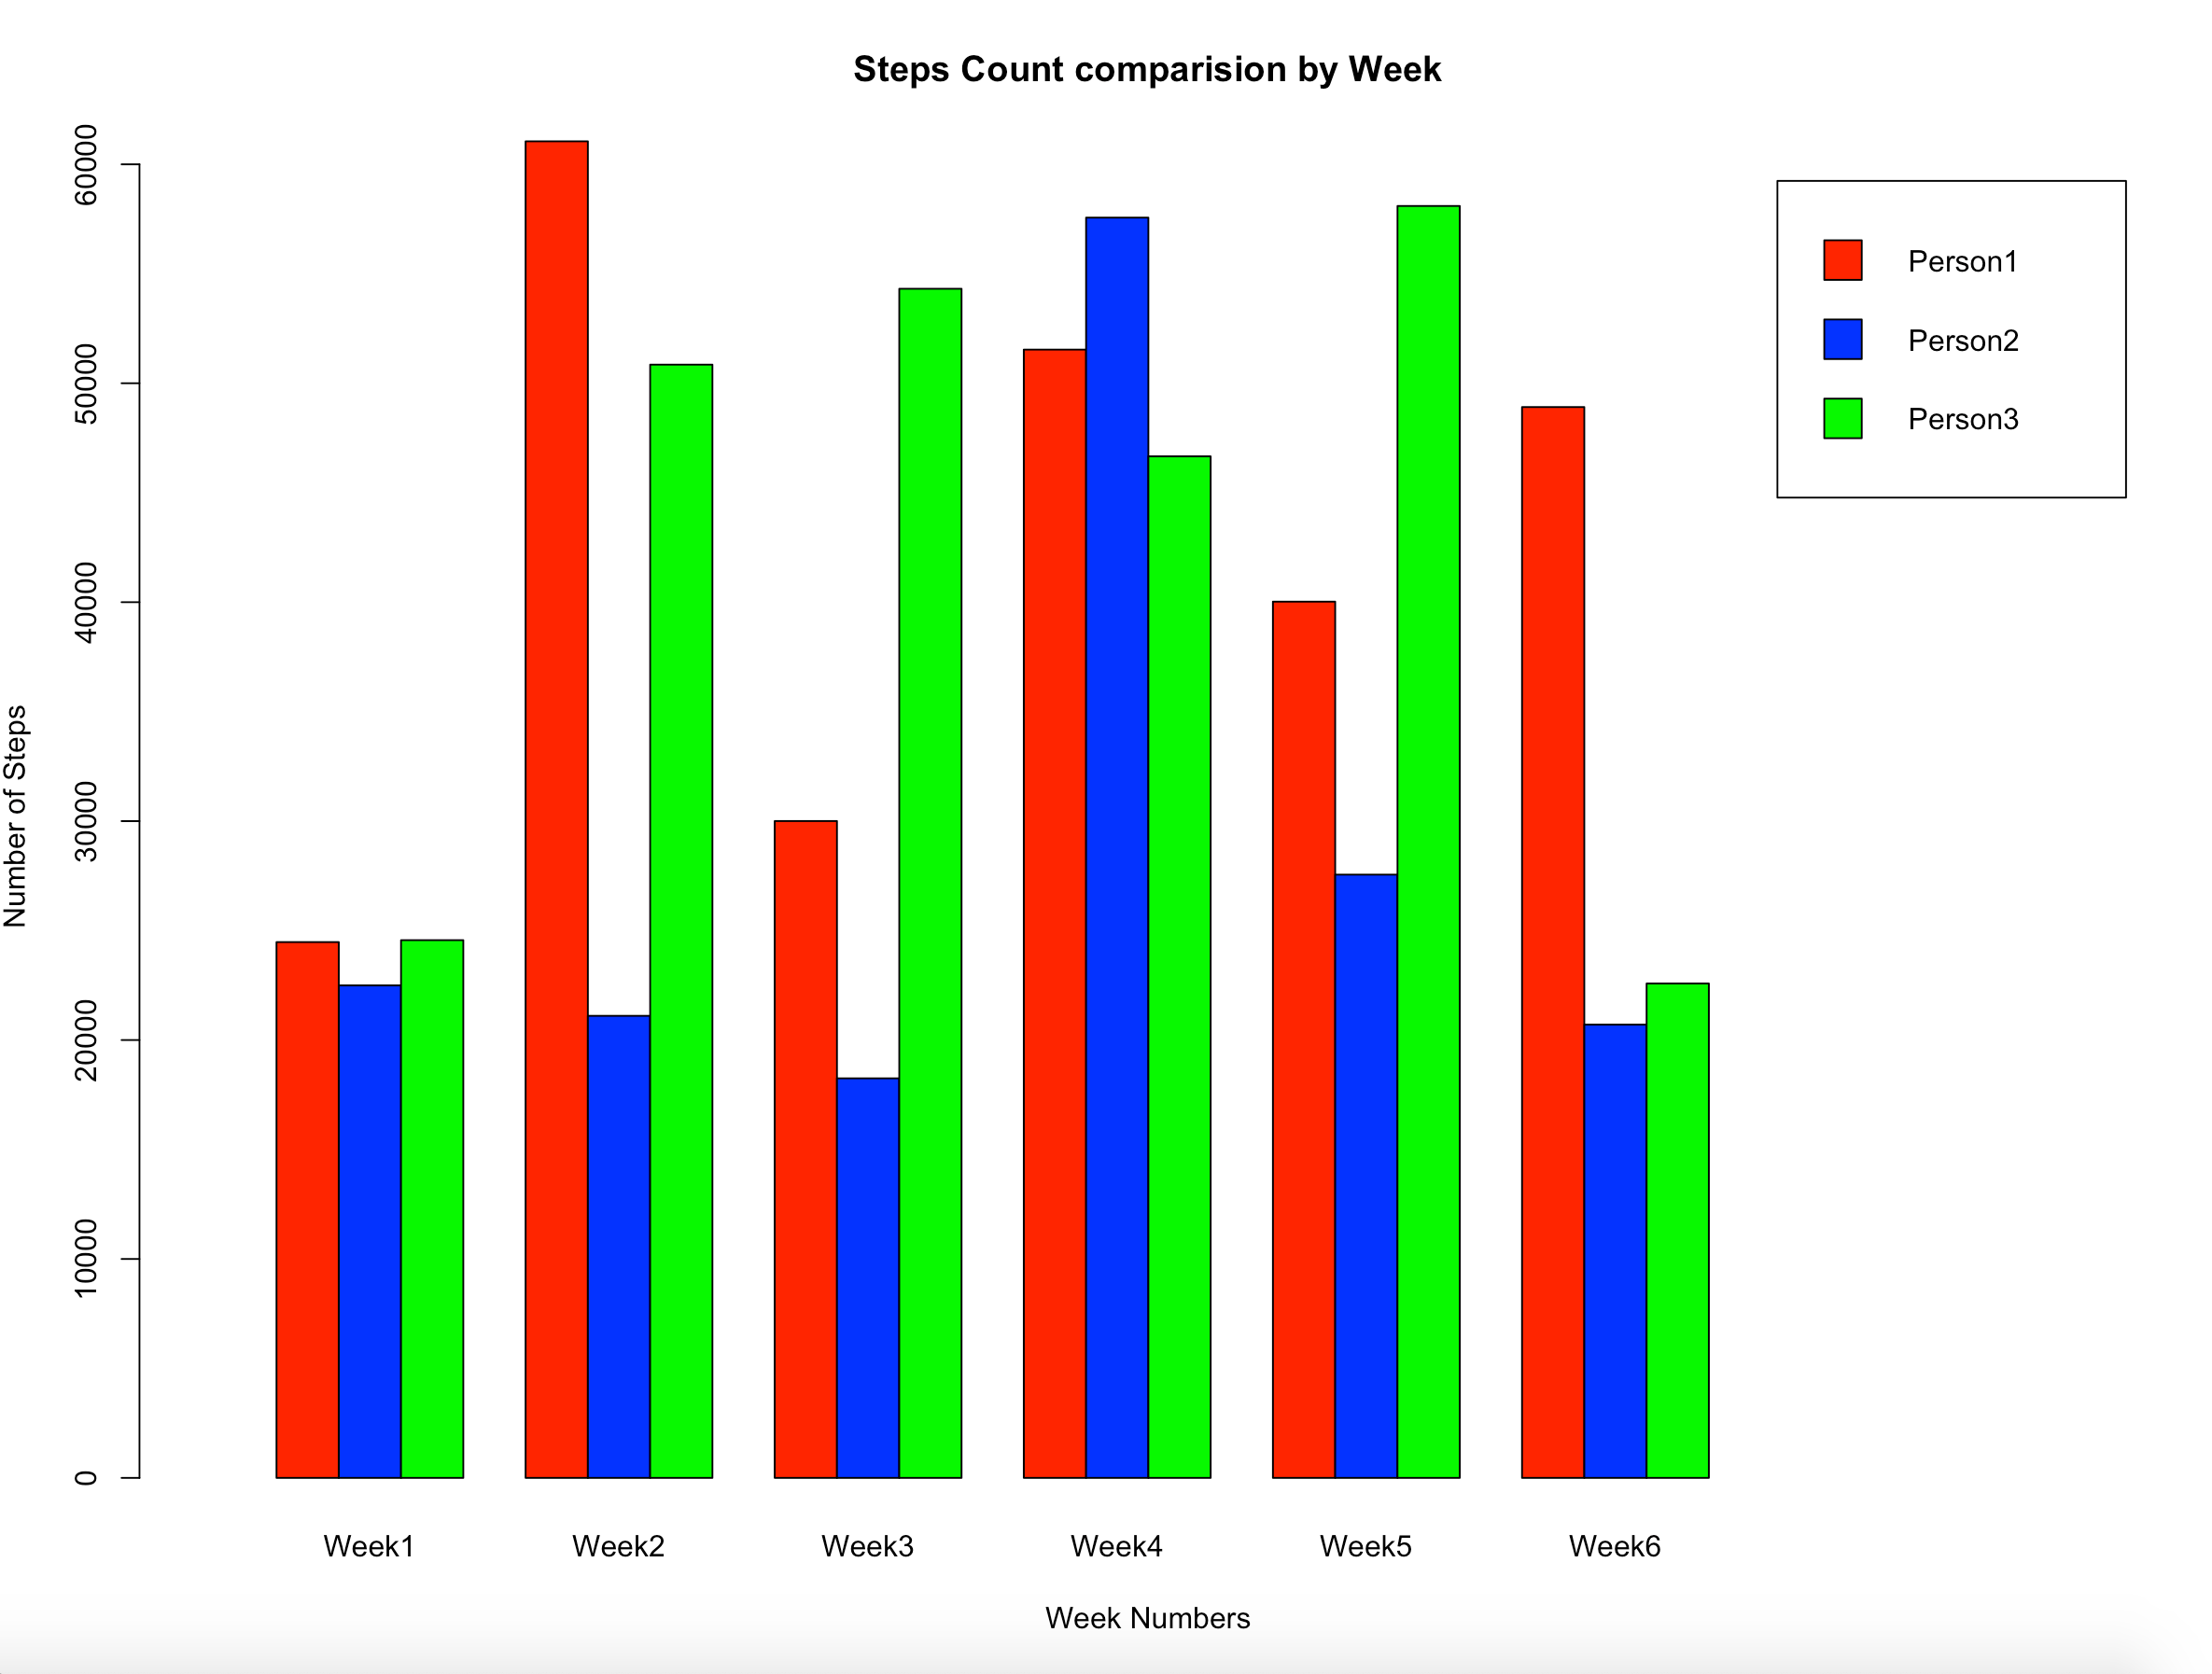
\includegraphics[width=0.6\linewidth]{/Users/abhisekgautam/Desktop/UTS/DSI/AT2//Screen Shot 2019-09-21 at 1.11.54 pm} 

}

\caption{\label{fig:figs}Figure 5: Steps Count of Group Members for different weeks}\label{fig:add_picture5}
\end{figure}

\hypertarget{steps-and-rainfall}{%
\subsection{4.3 Steps and Rainfall}\label{steps-and-rainfall}}

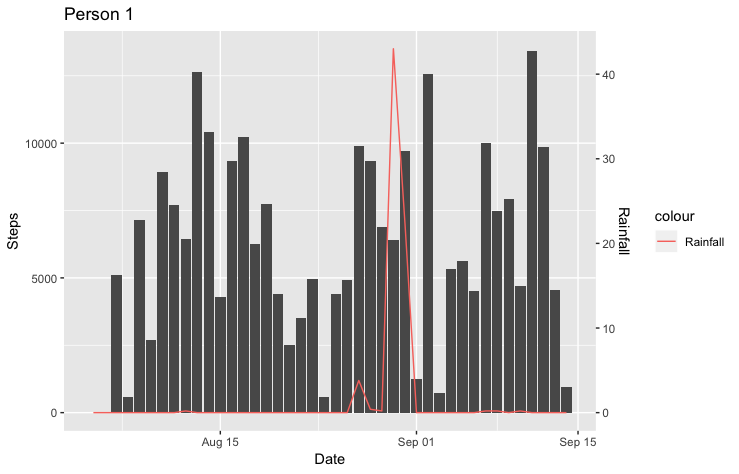
\includegraphics[width=0.5\linewidth]{/Users/abhisekgautam/Desktop/UTS/DSI/AT2//RainfallVsSteps_P1}
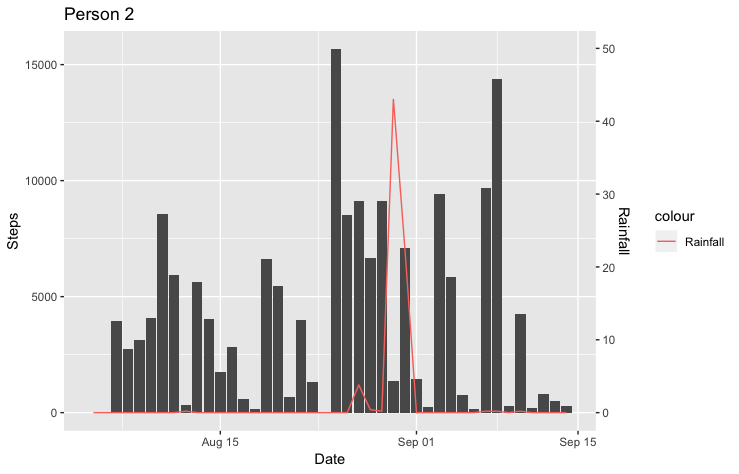
\includegraphics[width=0.5\linewidth]{/Users/abhisekgautam/Desktop/UTS/DSI/AT2//RainfallVsSteps_P2}

\begin{figure}

{\centering 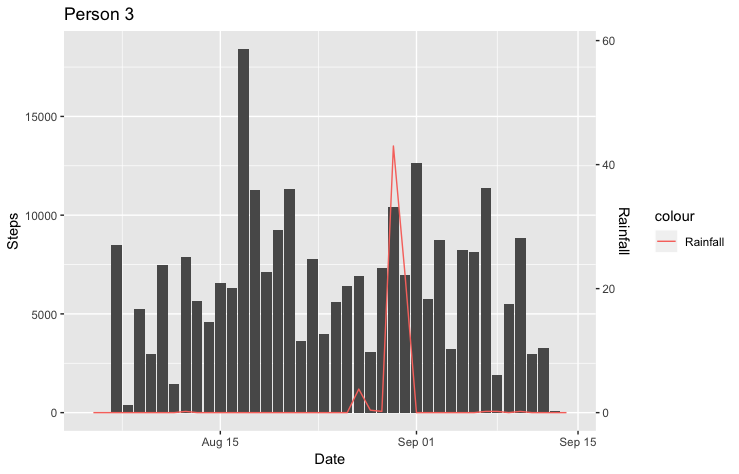
\includegraphics[width=0.5\linewidth]{/Users/abhisekgautam/Desktop/UTS/DSI/AT2//RainfallVsSteps_P3} 

}

\caption{\label{fig:figs}Figure 6: Rainfall vs. Steps count of Individual Members}\label{fig:image_graphs99}
\end{figure}

The plots in Figure 6 indicate that cohort is not particularly concerned
about walking when there is a rain. However, it is seems that Person2
had stayed at home during the heavy downpour on August 30th. Aug 31 also
had a bit of rain, but as there were classes, everybody had a
considerable number of steps.

\hypertarget{happiness-vs-steps}{%
\subsection{4.4 Happiness Vs Steps}\label{happiness-vs-steps}}

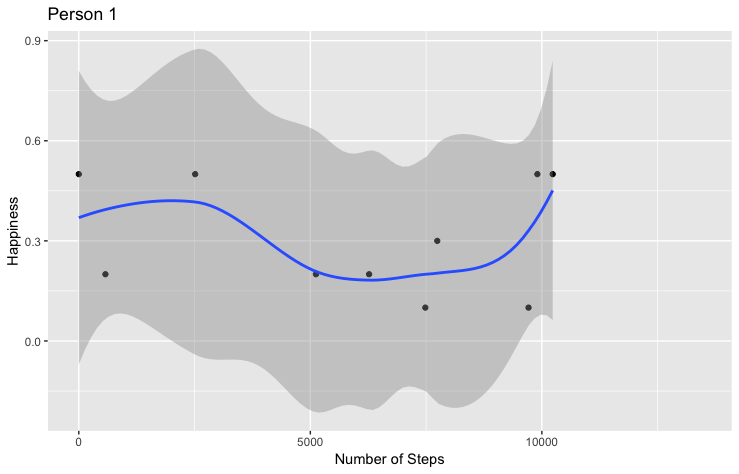
\includegraphics[width=0.5\linewidth]{/Users/abhisekgautam/Desktop/UTS/DSI/AT2//HappinessVSSteps_P1}
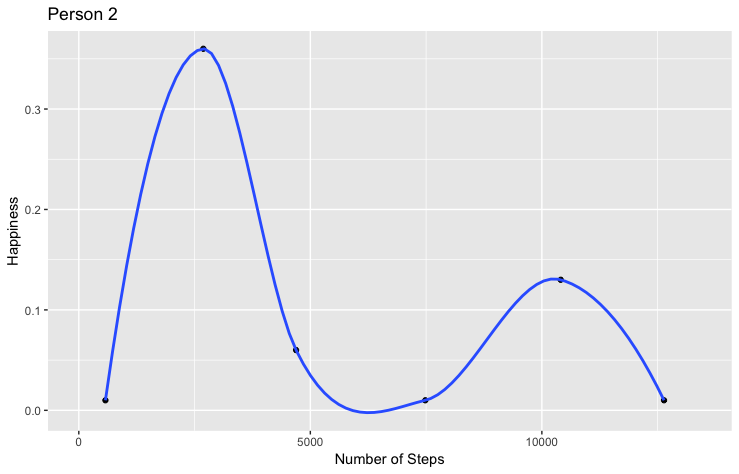
\includegraphics[width=0.5\linewidth]{/Users/abhisekgautam/Desktop/UTS/DSI/AT2//HappinessVsSteps_P2}

\begin{figure}

{\centering 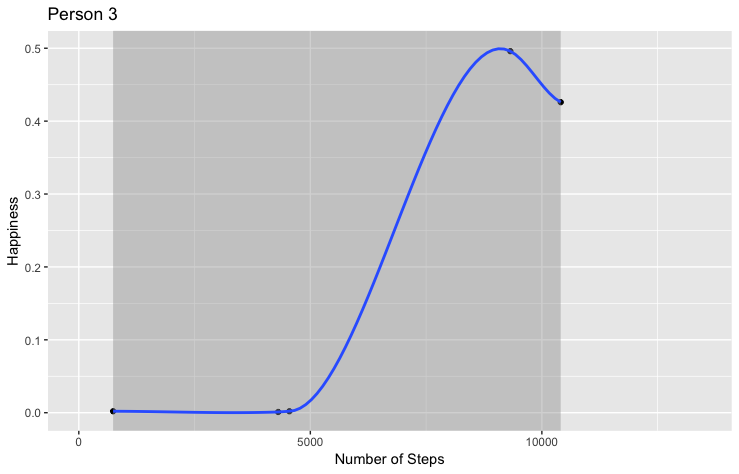
\includegraphics[width=0.5\linewidth]{/Users/abhisekgautam/Desktop/UTS/DSI/AT2//HappinessVsSteps_P3} 

}

\caption{\label{fig:figs}Figure 7: Happiness vs. Steps Count of Individual Members}\label{fig:image_graphs98}
\end{figure}

``Scientists say each step we take sends a boost of blood to our brains,
making us feel sharper and better overall'' (Horowitz, 2017). Though
there is very less data showing happiness from our moods, the plot of
Happiness and Steps Count indicates that Person1 and Person3 are happier
when they have more Steps Count. However, the claim is contradicted by
Person2's data which indicates that the person's happiness diminishes
when he/she walks more.

\hypertarget{individual-analysis}{%
\subsection{4.5 Individual Analysis}\label{individual-analysis}}

\begin{figure}

{\centering 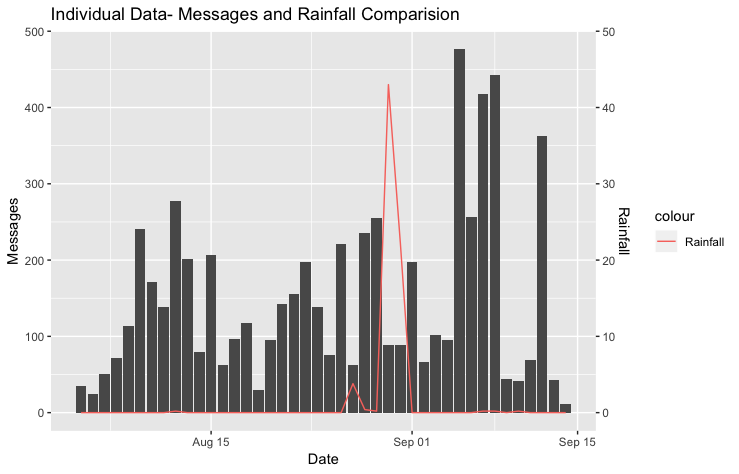
\includegraphics[width=0.6\linewidth]{/Users/abhisekgautam/Desktop/UTS/DSI/AT2//RainfallVsMessages} 

}

\caption{\label{fig:figs}Figure 8: Rainfall vs. Number of Messages}\label{fig:add_picture6}
\end{figure}

From Figure 8, it is clear that number of messages that are sent during
the peak rainfall is the least; around a hundred messages per day. My
personal preference during rainy days is to sit back and watch
television, so the figure could be indicating the same.

\begin{figure}

{\centering 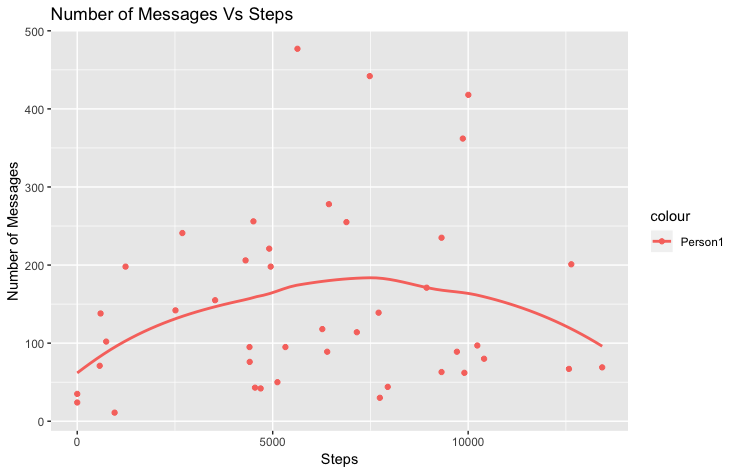
\includegraphics[width=0.6\linewidth]{/Users/abhisekgautam/Desktop/UTS/DSI/AT2//MessagesVsSteps} 

}

\caption{\label{fig:figs}Figure 9: Messages vs. Number of Steps}\label{fig:add_picture7}
\end{figure}

Figure 9 shows that I tend to be more active on social media when Steps
Count is between 5,000 to 10,000. The figure also indicates that more or
less steps than average implies less usage of Messenger.

This graph has inspired me to see another plot to check my steps count
according to days of the week.

\begin{figure}

{\centering 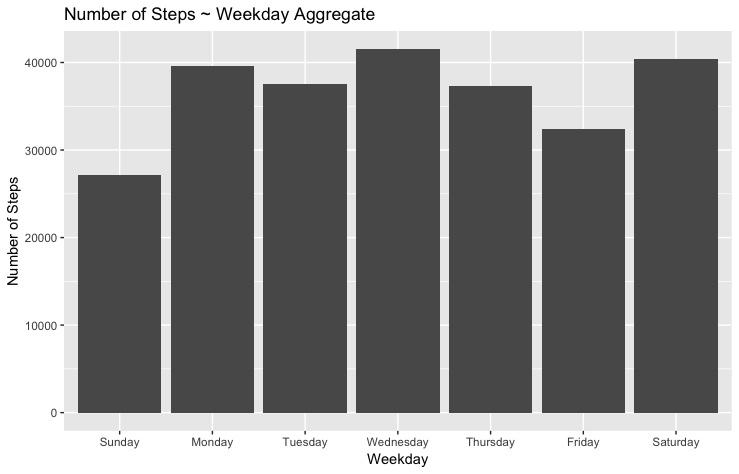
\includegraphics[width=0.6\linewidth]{/Users/abhisekgautam/Desktop/UTS/DSI/AT2//Day_of_week_steps} 

}

\caption{\label{fig:figs}Figure 10: Number of Steps according to Day of Week}\label{fig:add_picture8}
\end{figure}

Figure 10 shows the aggregated number of steps according to the week
day. It shows that the number of steps is less on Sundays, and the most
is on Wednesday. Sunday for me is a day to get household chores done,
rest and recharge myself for the upcoming week.

\hypertarget{ethical-privacy-and-legal-issues-of-the-collected-data}{%
\section{5. Ethical, Privacy and Legal Issues of the Collected
Data}\label{ethical-privacy-and-legal-issues-of-the-collected-data}}

Among collected data, GPS, Messenger and selfie phots leakage could lead
to legal issues. GPS and Messenger data can jeopardize a person's
privacy. In case of leakage of GPS data, a person may be stalked by
unwanted people. Messenger data leakage is has the capacity to break
relationships. Performing analytics on both the data could be used to
feed targeted advertisements to people, like the famous Facebook and
Cambridge Analytica data scandal (Meredith, 2018). Similarly, the issues
with selfie data is that it can be used to make fake videos of people
using artificial intelligence. Facial data ``can be used to create bogus
videos to defame someone, or potentially cause unrest by spreading
misinformation on a massive scale''(The Guardian, 2019). Besides these,
the steps count and weather data that are used in this report do not
have any privacy issues linked with them.

It is thus necessary to use protect data and use them ethically and
responsibly. In order to do that, we must make sure that the data that
is being used does not hamper the privacy of any other person. (Lee,
Wolfgang, \& Henry, 2016). Systems must be made secure and be protected
from unauthorized access and use. Also, there must be provisions of
registering rights to access publicly and privately owned data (Lee,
Wolfgang, \& Henry, 2016). The GPS data and Google Fit data used in this
study were collected from Google could only be extracted by the person
of the account. Also, Facebook's Messenger data could also be only
downloaded by the user. Both Facebook and Google required the user to
enter password while downloading them. In both their privacy policies,
it is written that the entire information could be accessed by
government if the user was a part of a government's investigation.

\hypertarget{discussion}{%
\section{6. Discussion}\label{discussion}}

This project started with mixed thoughts, and the group started looking
for data that could be collected, then built questions around them. It
would have been a better approach to do a preliminary research and then
form questions, followed by data collection. It is also sad to note that
during the middle of data collection, two group members dropped out from
the course, which impacted the quantity of data collected.

With a small amount of data, relationships were derived just sufficient
enough to hint an answer to the initial questions. Not much could be
concluded from the cohort's aggregated data. Stories were created around
the analysis to prove the correctness of data, and attempts were made to
generalize them.

Nevertheless, this project demended us to gather data, ask questions
based on the data, do analysis on it and find out the answers to those
questions; a key practice of Data Science. We initially had formulated a
list of questions that we were interested to look into in our life.
After that, data was collected to check on our questions, making
observations on a daily basis and implementing analytics on it, building
stories around the analyses and finally trying to answer the questions.

\hypertarget{reflection-and-conclusion}{%
\section{7. Reflection and Conclusion}\label{reflection-and-conclusion}}

This project has made me realize the power of data and how it can be
interpreted and used in personal reflection. There are a lot of factors
in our daily life that drive our behaviours, and we tend to ignore them
while going through our days. We all would like to be a better version
of ourselves, but we are not keeping notice about the minor things that
change our behaviour. If we know what we have been doing till date, it
will be easy to change some of them and observe their effect on us.
Repeated test and observation on ourselves will make sure that we
improve our behaviours that go unnoticed. I have seen that our
behaviours can be anticipated by data, and with the control over our
data, we can control our behaviours.

The project has helped me understand about the of people in my group as
well as my individual behaviour. Some of the findings that were not so
abvious in our group were found, such as a member in our group who is
seen to walk only when there are classes, else he sits at home. It was
observed to the remaining two members that they had higher probability
of being happy if they walked more during the day. In my case, I have
come to know that one day in a week (mostly Sunday), I do not walk much.
Also, I am somewhat aware about in what contexts my usage of Messenger
varies. By knowing these small things about my life, it can be helpful
if I wanted to change something that is going on in my life.
Additionally, this project has encouraged me to think about and collect
other types of data so that I can know more about myself.

If this project were to be done again, different sets of data would be
taken. Data related to food intake, calorie lost during exercise and
sleep patterns would be the best to analyse in my opinion. The GPS data,
though was accurate, could not be much of a use in quantifying self
except plotting it into a map. Also, more reliable devices such as
fitness tracker would be used from next time to track steps and motion
more accurately. Lastly, instead of selfies, journal entries would have
been a more accurate way to measure the sentiments.

\hypertarget{references}{%
\section{8. References}\label{references}}

Quantified Self Institute, 2017, \emph{What is quantified self?}, viewed
on 20 September 2019,
\url{https://qsinstitute.com/about/what-is-quantified-self/}

Ferris, T., \emph{The First-Ever Quantified Self Notes (Plus: LSD as
Cognitive Enhancer?)}, viewed on 20 September 2019,
\url{https://tim.blog/2013/04/03/the-first-ever-quantified-self-notes-plus-lsd-as-cognitive-enhancer/}.

Lee, W. W., Z. Wolfgang and C. Henry, 2016, \emph{An Ethical Approach to
Data Privacy Protection},ISACA Journal, Volume 6, 2016, viewed on 21
September 2019,
\url{https://www.isaca.org/Journal/archives/2016/volume-6/Pages/an-ethical-approach-to-data-privacy-protection.aspx}

Swan, M., 2013, \emph{The Quantified Self: Fundamental Disruption in Big
Data Science and Biological Discovery}, viewed on 25th October, 2019,
\url{https://www.liebertpub.com/doi/full/10.1089/big.2012.0002}

\emph{Data Policy, Facebook}, viewed on 26th October 2019,
\url{https://www.facebook.com/policy.php}

\emph{Terms and Conditions, Google Fit}, viewed on 26th October 2019,
\url{https://developers.google.com/fit/terms}

Horowitz, K., 2017, \emph{Why Walking Makes Us Feel Good}, viewed on
27th October 2019,
\url{http://mentalfloss.com/article/94677/why-walking-makes-us-feel-good}

Meredith, S., 2018, \emph{Here's everything you need to know about the
Cambridge Analytica scandal}, viewed on 27th October 2019,
\url{https://www.cnbc.com/2018/03/21/facebook-cambridge-analytica-scandal-everything-you-need-to-know.html}

The Guardian, 2019, \emph{Chinese deepfake app Zao sparks privacy row
after going viral}, viewed on 27th October 2019,
\url{https://www.theguardian.com/technology/2019/sep/02/chinese-face-swap-app-zao-triggers-privacy-fears-viral}

\hypertarget{appendix}{%
\section{9. Appendix}\label{appendix}}

\hypertarget{correlations-in-group-data}{%
\subsection{9.1 Correlations in Group
Data}\label{correlations-in-group-data}}

\begin{figure}

{\centering 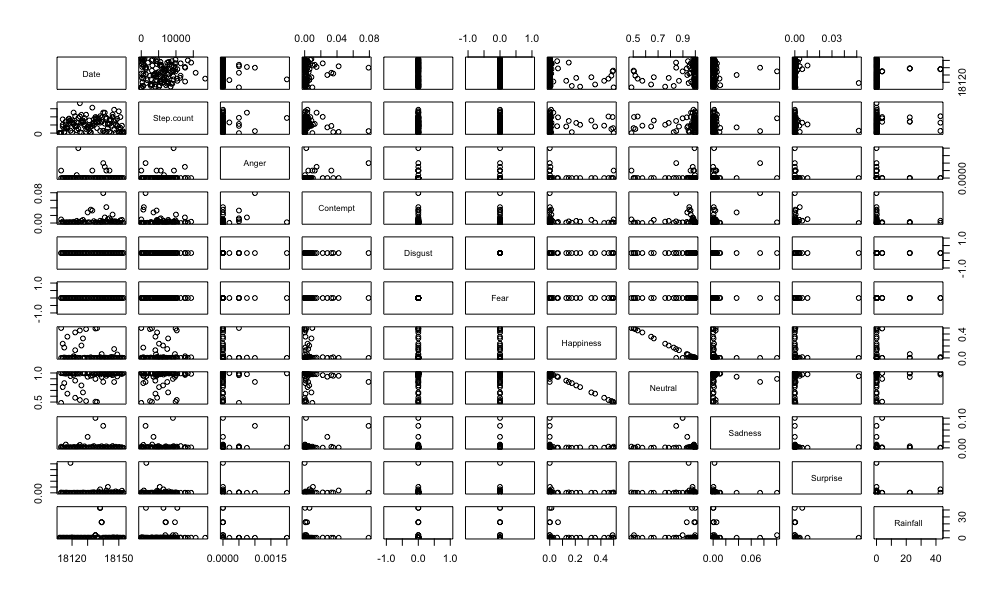
\includegraphics[width=1\linewidth]{/Users/abhisekgautam/Desktop/UTS/DSI/AT2//Plot_all} 

}

\caption{\label{fig:figs}Appendix 1: Correlations in Group Data}\label{fig:add_picture97}
\end{figure}

\hypertarget{correlations-in-individual-data}{%
\subsection{9.2 Correlations in Individual
Data}\label{correlations-in-individual-data}}

\begin{figure}

{\centering 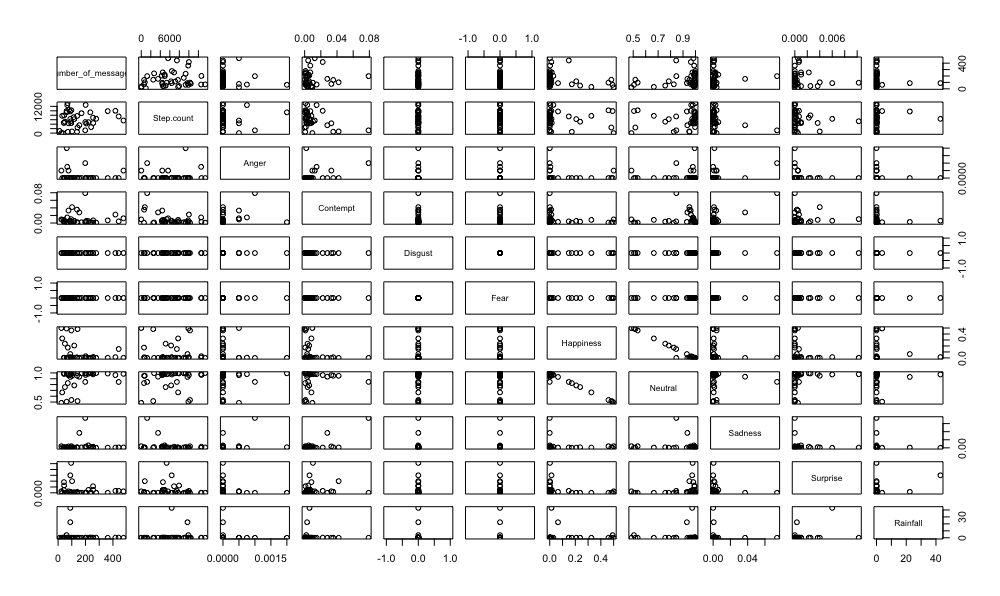
\includegraphics[width=1\linewidth]{/Users/abhisekgautam/Desktop/UTS/DSI/AT2//Individual_Summary_corr} 

}

\caption{\label{fig:figs}Appendix 2: Correlations in Individual Data}\label{fig:add_picture96}
\end{figure}

\hypertarget{mood-data-scatter-plots}{%
\subsection{9.3 Mood Data Scatter Plots}\label{mood-data-scatter-plots}}

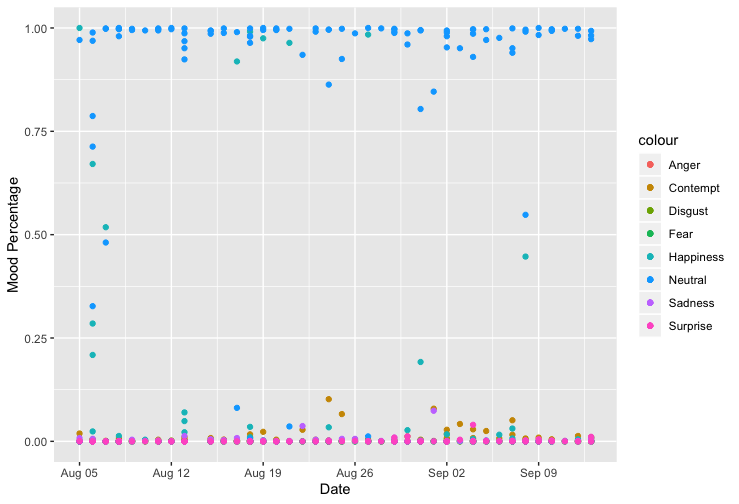
\includegraphics[width=0.5\linewidth]{/Users/abhisekgautam/Desktop/UTS/DSI/AT2//Mood_P1}
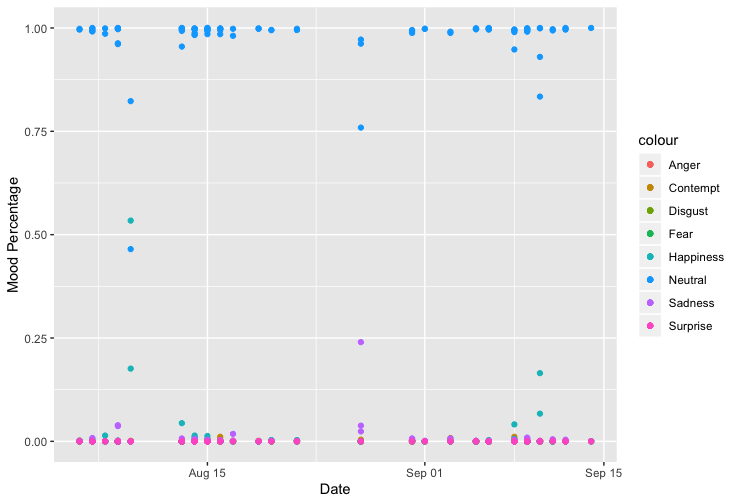
\includegraphics[width=0.5\linewidth]{/Users/abhisekgautam/Desktop/UTS/DSI/AT2//Mood_P2}

\begin{figure}

{\centering 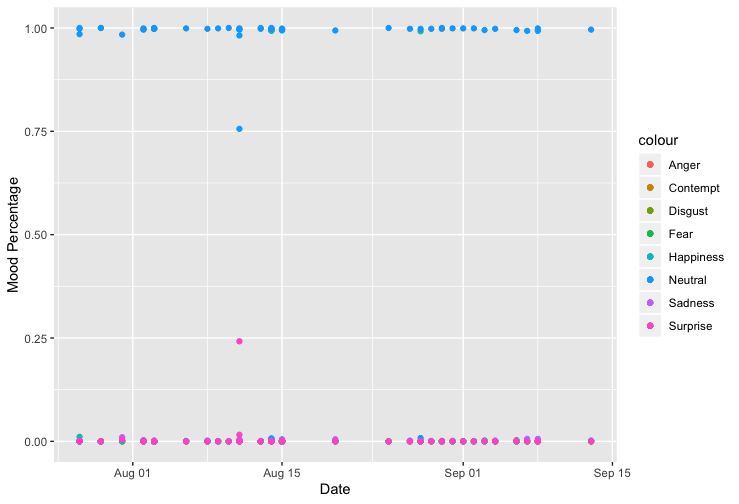
\includegraphics[width=0.5\linewidth]{/Users/abhisekgautam/Desktop/UTS/DSI/AT2//Mood_P3} 

}

\caption{\label{fig:figs}Appendix 3: Mood Data Scatter Plots}\label{fig:add_picture94}
\end{figure}

\end{document}
